\section{为什么需要维数公式？}
\label{sec:dim-motivation}
% ============================================================================

一上来先看一串很像“魔法”的数字：
\[
  \dim \Mk_k(\SL_2(\Z))=
  \begin{cases}
    0,& k<0\text{ 或 }k\text{ 为奇数},\\
    1,& k=0,4,6,8,10,\\
    0,& k=2,\\
    2,& k=12,\\
    \dots
  \end{cases}
\]
而尖点形式空间又给出另一串数字：
\[
  \dim \Sk_{12}=1,\qquad
  \dim \Sk_{16}=\dim \Sk_{18}=\dim \Sk_{20}=\dim \Sk_{22}=1,\qquad
  \dim \Sk_{24}=2.
\]

这些数值背后显然有规律，但若只靠逐个构造 Eisenstein 级数、逐个找 cusp form，规律很难看清。我们真正想问的是：

\begin{quote}
\emph{为什么偏偏是这些数字？它们能不能由一条统一的几何公式直接算出来？}
\end{quote}

答案是：可以，而核心工具正是上一章刚出现的紧模曲线 $X(\Gamma)$ 与 Riemann--Roch 定理。也就是说，维数公式不是“又一串特殊函数恒等式”；它是\textbf{把模形式空间翻译成曲线上的线丛截面空间，再用代数几何数截面}的结果。

\textbf{维数为什么重要？} 因为它直接决定我们接下来能做什么。
\begin{itemize}
  \item 若 $\dim \Sk_k=1$，那么这个空间中的任一非零向量都自动是 Hecke 特征形式。例如
        $\Sk_{12}(\SL_2(\Z))=\C\Delta$，所以 $\Delta$ 不需要再对角化，天然就是特征形式。
  \item 若 $\dim \Sk_k=2$，事情就立刻变得更有趣：空间里通常会分裂出两条 Hecke 特征线，需要把 Hecke 算子真正对角化。
  \item 维数还是“唯一性”的上界信息。粗略地说，若一个空间只有有限维，那么给出足够多个 Fourier 系数就能唯一确定一条模形式；这正是后面比较模形式、证明恒等式时的基本策略。
\end{itemize}

先把最常见的一张表列出来。它是本章全部内容要解释的对象：

\begin{center}
\begin{tabular}{c|cccccccccccc}
\toprule
$k$ & 4 & 6 & 8 & 10 & 12 & 14 & 16 & 18 & 20 & 22 & 24 & 26 \\
\midrule
$\dim \Mk_k$ & 1 & 1 & 1 & 1 & 2 & 1 & 2 & 2 & 2 & 2 & 3 & 2 \\
$\dim \Sk_k$ & 0 & 0 & 0 & 0 & 1 & 0 & 1 & 1 & 1 & 1 & 2 & 1 \\
\bottomrule
\end{tabular}
\end{center}

% figures/ch03-dimension-chart.tex
% Chapter 5: dimensions of cusp forms for SL_2(Z)
\begin{figure}[ht]
\centering
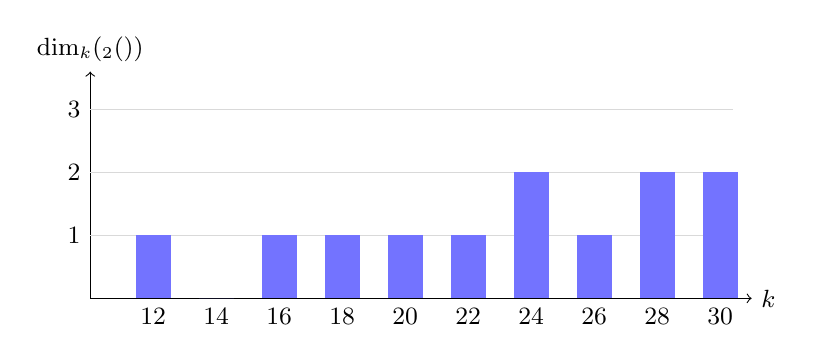
\begin{tikzpicture}[x=0.8cm,y=0.8cm,font=\small]
  \draw[->] (0,0) -- (10.5,0) node[right] {$k$};
  \draw[->] (0,0) -- (0,3.6) node[above] {$\dim \Sk_k(\SL_2(\Z))$};

  \foreach \x/\k in {1/12,2/14,3/16,4/18,5/20,6/22,7/24,8/26,9/28,10/30}
    \node[below] at (\x,0) {\k};

  \foreach \y in {1,2,3}
    {\draw[gray!30] (0,\y) -- (10.2,\y); \node[left] at (0,\y) {\y};}

  \foreach \x/\h in {1/1,2/0,3/1,4/1,5/1,6/1,7/2,8/1,9/2,10/2}
    \fill[blue!55] (\x-0.28,0) rectangle (\x+0.28,\h);
\end{tikzpicture}
\caption{$\SL_2(\Z)$ 上尖点形式空间维数的前几个值。最早出现的非零空间是 $\Sk_{12}=\C\Delta$；之后维数按“每跨过一个 $12$ 就大致增加 $1$”的节奏增长。}
\label{fig:dimension-chart}
\end{figure}


这张表里有三件事尤其值得记住。
\begin{enumerate}
  \item \textbf{第一个 cusp form 出现在权 $12$。} 这不是偶然；它反映了 valence formula 中“总零点数等于 $k/12$”的门槛现象。
  \item \textbf{大致每跨过一个 $12$，维数就增加 $1$。} 因为乘上 $\Delta$ 会把权从 $k-12$ 提升到 $k$，并把模形式送到尖点形式。
  \item \textbf{$k\equiv 2\pmod{12}$ 时会少一维。} 这正是椭圆点 $i,\rho$ 的局部行为留下的“修正项”。
\end{enumerate}

本章的路线图也因此很自然：
\begin{itemize}
  \item 先用 Riemann--Roch 解释“为什么维数问题本质上是线丛截面计数”；
  \item 再完整算出 $\SL_2(\Z)$ 的维数公式；
  \item 最后推广到 $\Gamma_0(N)$ 等一般同余子群，并把公式真正用在具体级别上。
\end{itemize}

读完整章后，像“$\dim \Sk_{12}=1$ 所以 $\Delta$ 自动是特征形式”“$\dim \Sk_2(\Gamma_0(11))=1$ 所以权 $2$ 新形式唯一”这样的断言，就不再像魔法，而会变成直接可算的结论。
